% !TEX root =  ../conclusions.tex
\section{Conclusions}

% What are your main conclusions from these results?
% This section should lead from the Results into the Improvements.
% Describe how you will improve our application based on your results. What changes will you make, and why? What would it look like before and after? Why is the improved version better? Motivate your choices using the heuristics and your results.
% The conclusion of this section should show your final GUI design.
% Note that this report is only about the design, so it is not necessary to already show the finished improved implementation.

Our main conclusions from the results were that the issues found could be summarised as a mix of lacking implementations, technical bugs, and exposing technical details to the user that could use a layer of indirection or translation from technical jargon to layman English. Lastly, some navigation elements were hard to spot or not traversable with shortcuts

\subsection{Improvements}

"Missing features and bugs were straightforward enough - they simply needed to be coded. Having the UI suggest features that did not exist and having bugs was extremely confusing and was not acceptable. Secondly, having error messages at all would be minimized in favour of using GUI to, for instance, highlight fields with invalid input in red or show tool-tips. Nielsen's 5th heuristic detailed this. In some places, error messages were necessary, for instance, when the error was network-related. In that case, the error messages would appear in custom windows with a style that was in line with the rest of the app and in plain English. Any unexpected errors simply showed as "Something went wrong. That’s all we knew.""
The last thing was a GUI overhaul - the design needed to be more aesthetically pleasant, and most crucially, clear, in line with Nielsen’s 8th heuristic. "Back" buttons needed to be ubiquitous, large, and visible. Lastly, the team decided to also satisfy the second heuristic, "Match between the system and the real world." This will show in the final GUI design.


\subsection{Final Design}

Firstly, the navigation of the system is laid out in this illustration.

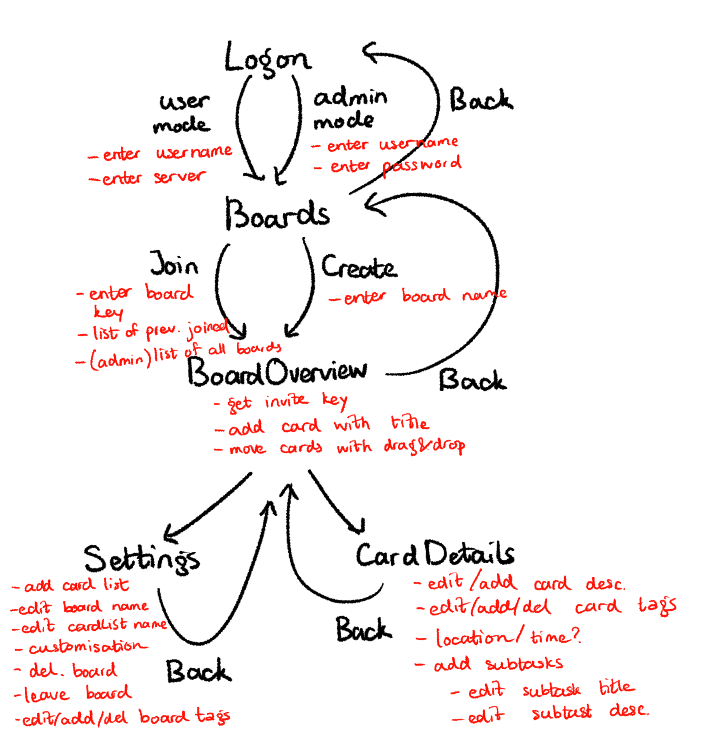
\includegraphics{mocks/hue_mock_flow.png}

\textbf{Figure 6: A "sitemap" of the application.}
\newline

The new GUI aims to use a pop-art, 90's high school sports style to tie the design together. The colours were chosen to contrast strongly, but the background uses a light gradient to smooth it all together as to not be too overwhelming. The navigation buttons are extremely large and contrast heavily to make sure the use does not miss them.

A series of sketches that show that illustrate the idea of the design will follow. This design might not be implemented in the final product. 

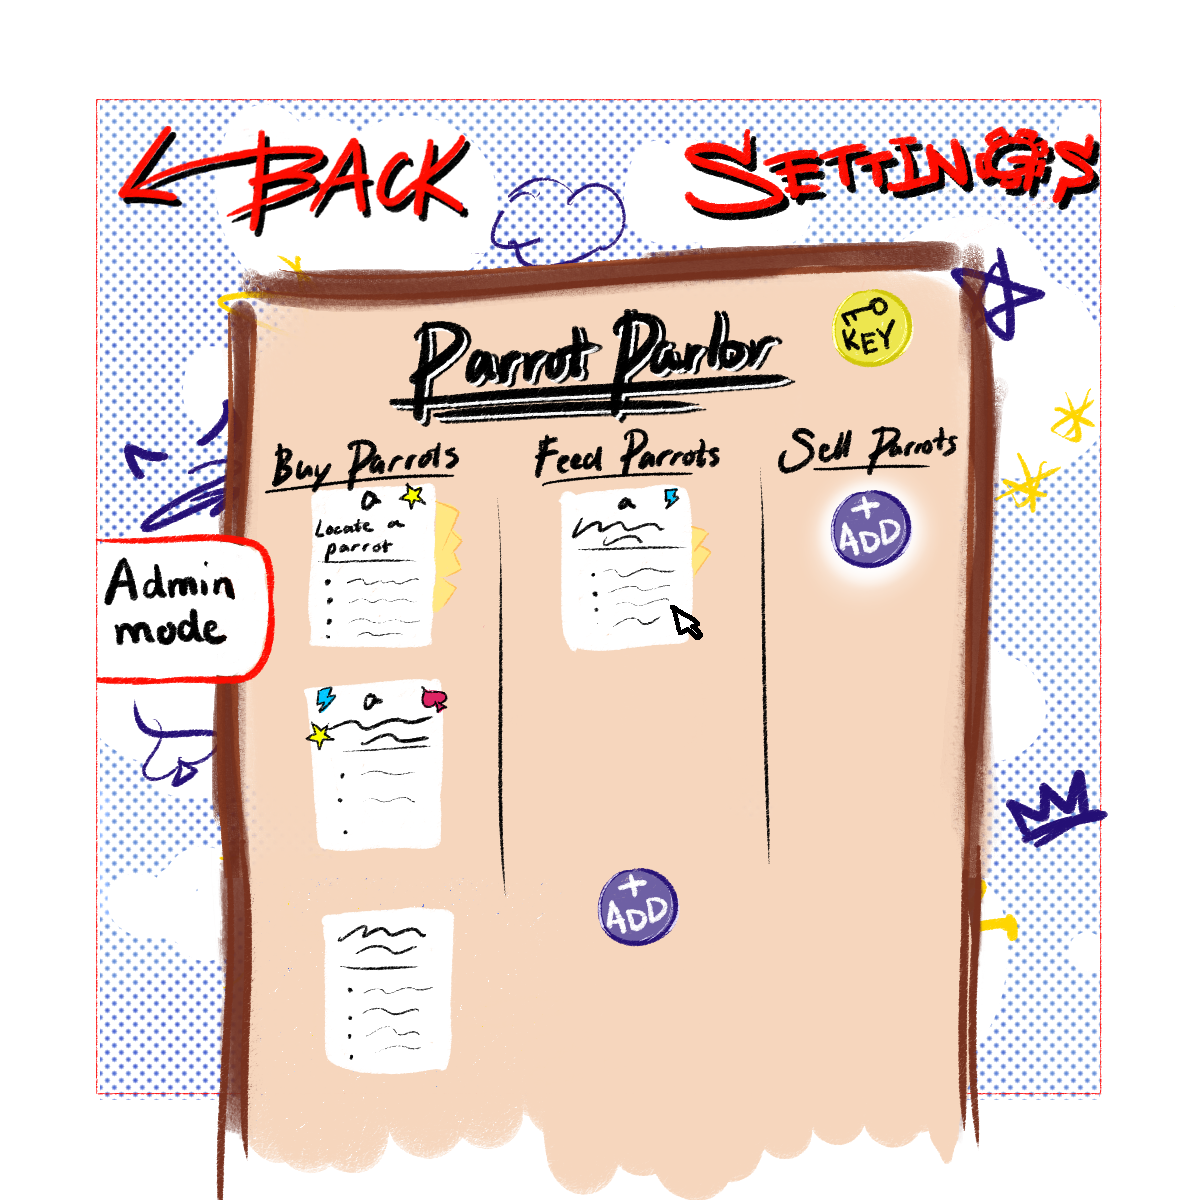
\includegraphics[scale=0.8]{mocks/hue_mock_board_overview.png}
\textbf{Figure 7: The board overview screen.}
\newline

This is the main screen. It aims to visually mimic a community board on a wall, using A4 paper sheets as Card designs, and Post-it notes for sub-tasks. The buttons are designed to mimic button-pins. This screen hides a lot of information such as the sub-task texts and the tag names, in line with Nielsen's 8th heuristic. Instead, it uses colourful shapes to communicate the presence of tags, and shows small bits of Post-it hiding from behind a Card to show how many sub-tasks there are, without showing what they are. This card-specific information can be accessed from the Card Details screen. When adding more Cards than fit on the screen, a vertical scroll-bar appears on hover.

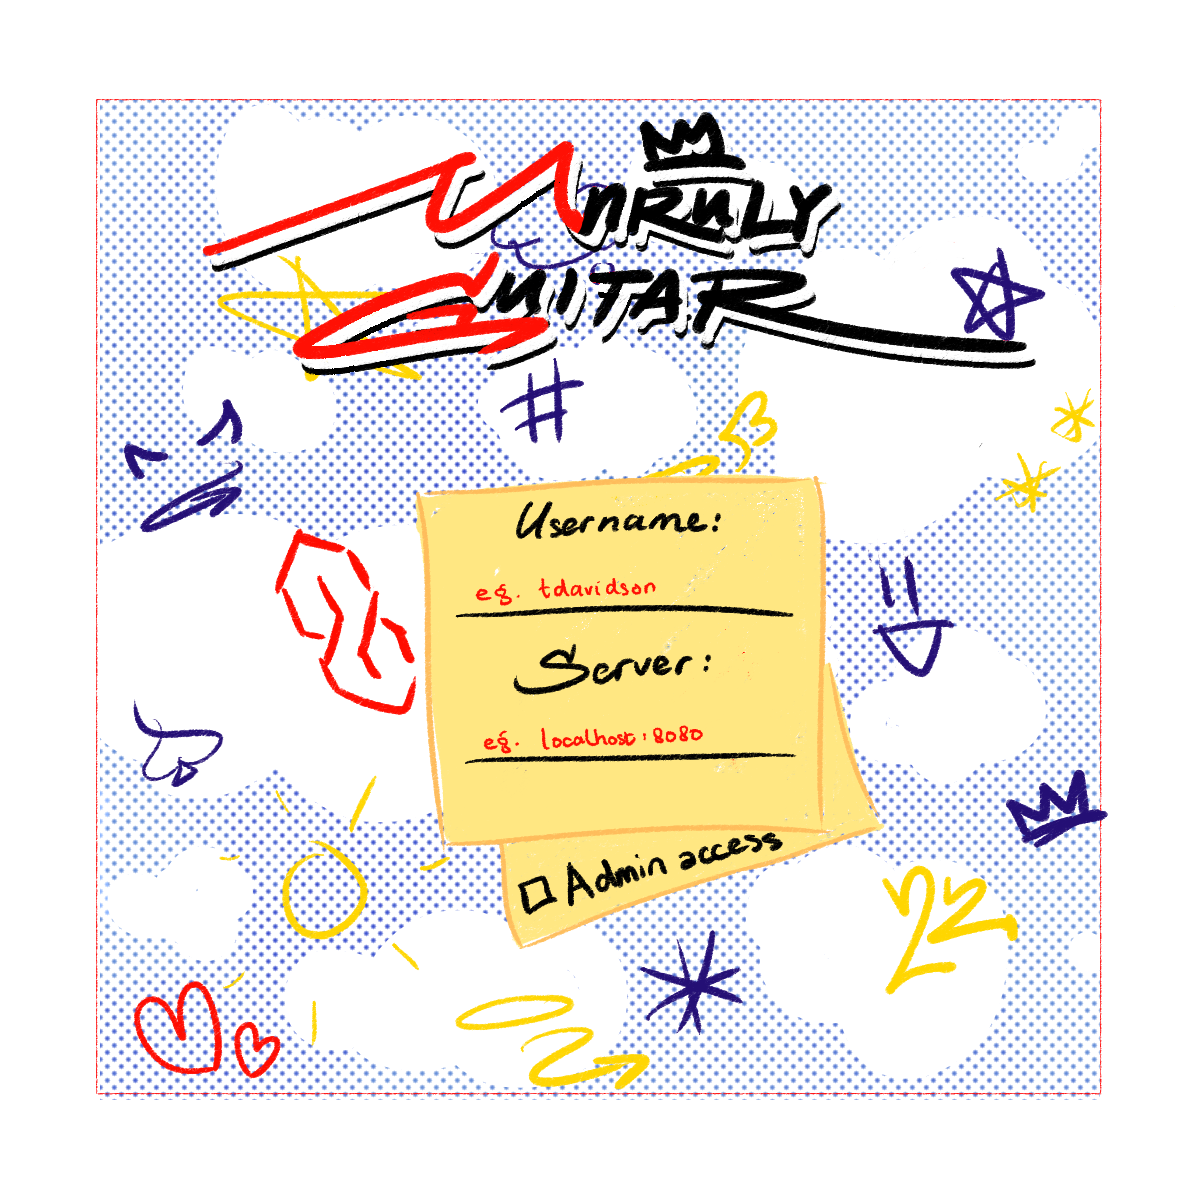
\includegraphics[scale=0.8]{mocks/hue_mock_logon.png}
\textbf{Figure 8: The logon screen.}
\newline

This screen includes the logo, using Post-it notes again to communicate input forms with few fields. The idea is to use a slide-out animation that reveals the admin password field when admin access is requested.

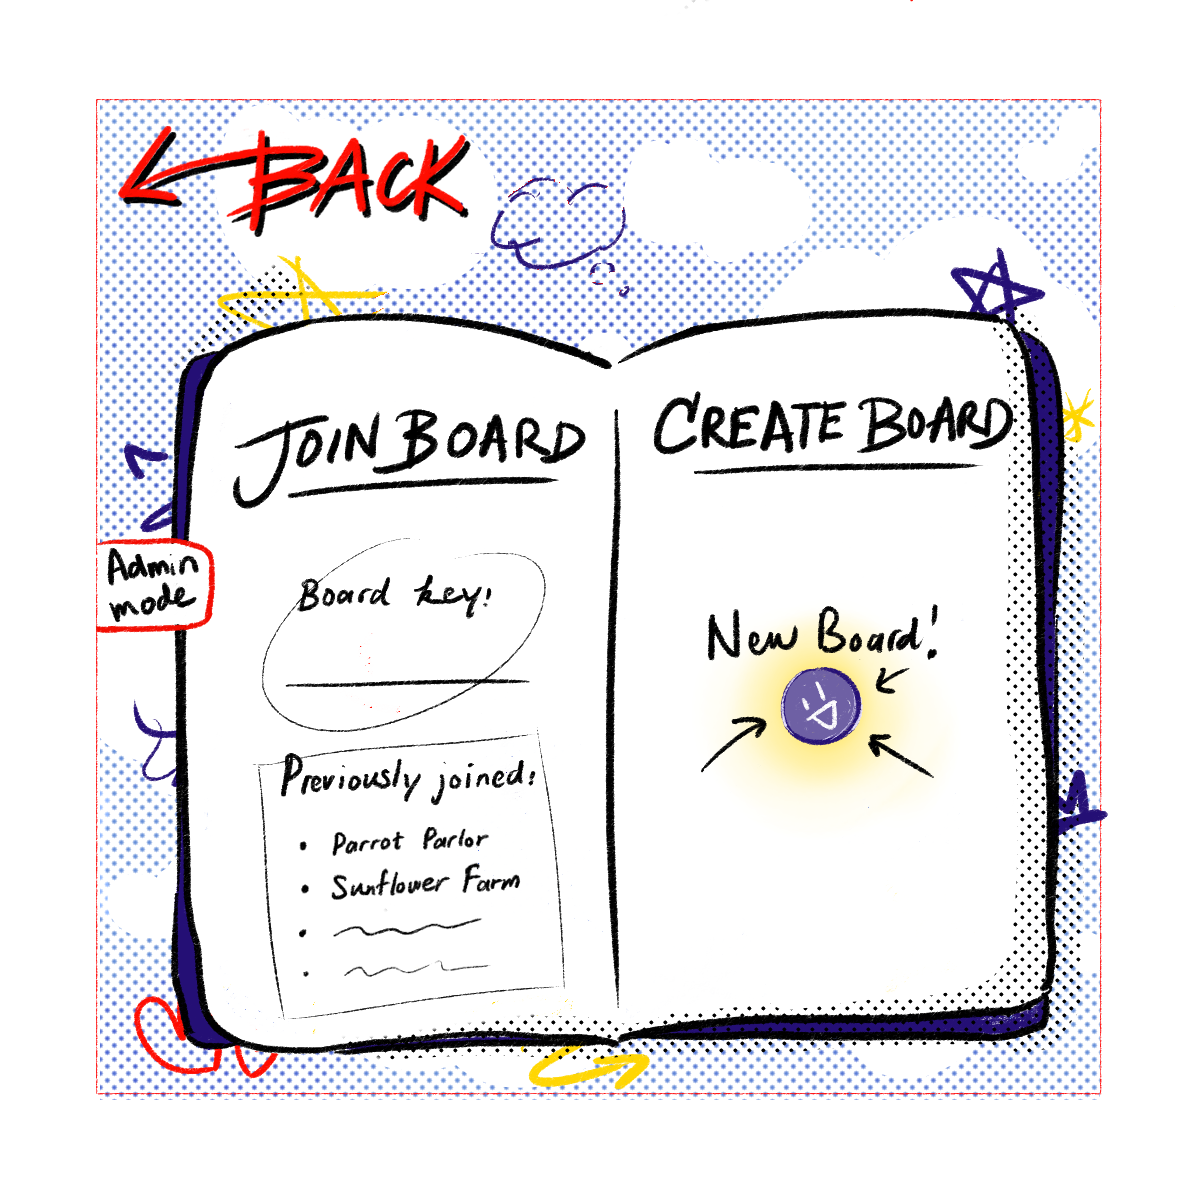
\includegraphics[scale=0.8]{mocks/hue_mock_boards.png}
\textbf{Figure 9: The boards screen.}
\newline

This screen uses skeuomorhpism again to imitate a notebook of sorts. More half-tone dots are used for shading, to really push the pop-art style.

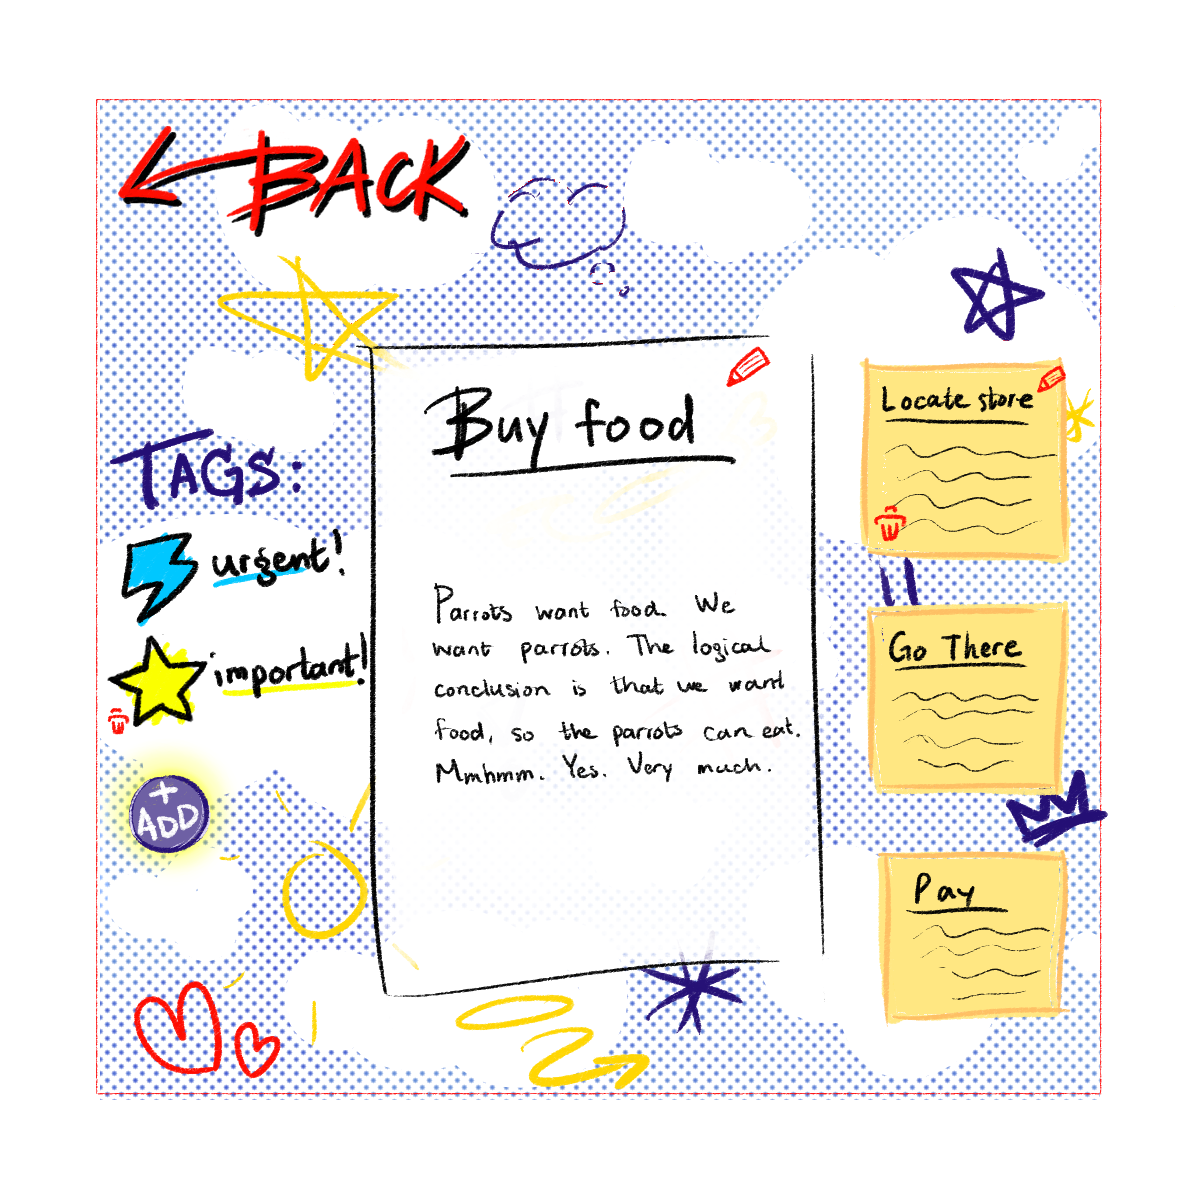
\includegraphics[scale=0.8]{mocks/hue_mock_card_details.png}
\textbf{Figure 10: The card details screen.}
\newline

On hover, small pencil or trashcan icons appear to remind the user of the editing functionality with icons that are commonly used in other applications, in line with the 6th heuristic. On this screen, subtask titles and descriptions are shown, as well as tag names, which were not shown on the board overview screen. When adding more sub-tasks than fit on the screen, a horizontal scroll-bar appears on hover.